\documentclass{standalone}
%\documentclass[convert={density=600,size=1080x800,outext=.png}]{standalone}
%\documentclass[convert={outext=.jpg}]{standalone}
\NeedsTeXFormat{LaTeX2e}
\usepackage{tikz}
\usepackage[utf8]{inputenc}
\usepackage{wasysym}
\usepackage{gensymb}
% \usepackage{fontspec}

\newcommand\Name{Ekosfera/1903} % Name
\newcommand\Crystal{INTRI-7201} % Crystal number
\newcommand\HEAD{1.35} % HEAD conc x 10^10
\newcommand\TAIL{1.70} % TAIL conc x 10^10
\newcommand\Scale{4} % Scale
\newcommand\Dia{52.2} % Detector diameter in mm
\newcommand\Hei{42.9} % Detector hight in mm
\newcommand\Gdt{5} % Groove depth
\newcommand\Bult{3} %widow bulletization
\newcommand\Cdiam{8.5} %Contact diam 
\newcommand\Cdepth{28.4} %Contact depth
\newcommand\GrvEx{27.5} %Groove ext. diameter
\newcommand\GrvIn{17.5} %Groove int. diameter



\newcommand\Diam{\Dia/\Scale} % Detector diameter in mm
\newcommand\Height{\Hei/\Scale} % Detector hight in mm
\newcommand\WO{\Gdt/\Scale} % Groove depth
\newcommand\Bullet{\Bult/\Scale} %widow bulletization
\newcommand\FCD{\Cdiam/\Scale} %Contact diam 
\newcommand\CDepth{\Cdepth/\Scale} %Cont depth
\newcommand\GrooveExt{\GrvEx/\Scale} %Groove ext. diameter
\newcommand\GrooveInt{\GrvIn/\Scale} %Groove int. diameter

\tikzset{
  arrow/.style={<->,>=latex,thin,gray,every rectangle node/.style={fill=white,midway,font=\sffamily}},
  dimen/.style={thin,gray},
  caption/.style={font=\sffamily,gray},
  lithium/.style={red!90!white,ultra thick},
}
\begin{document}

    
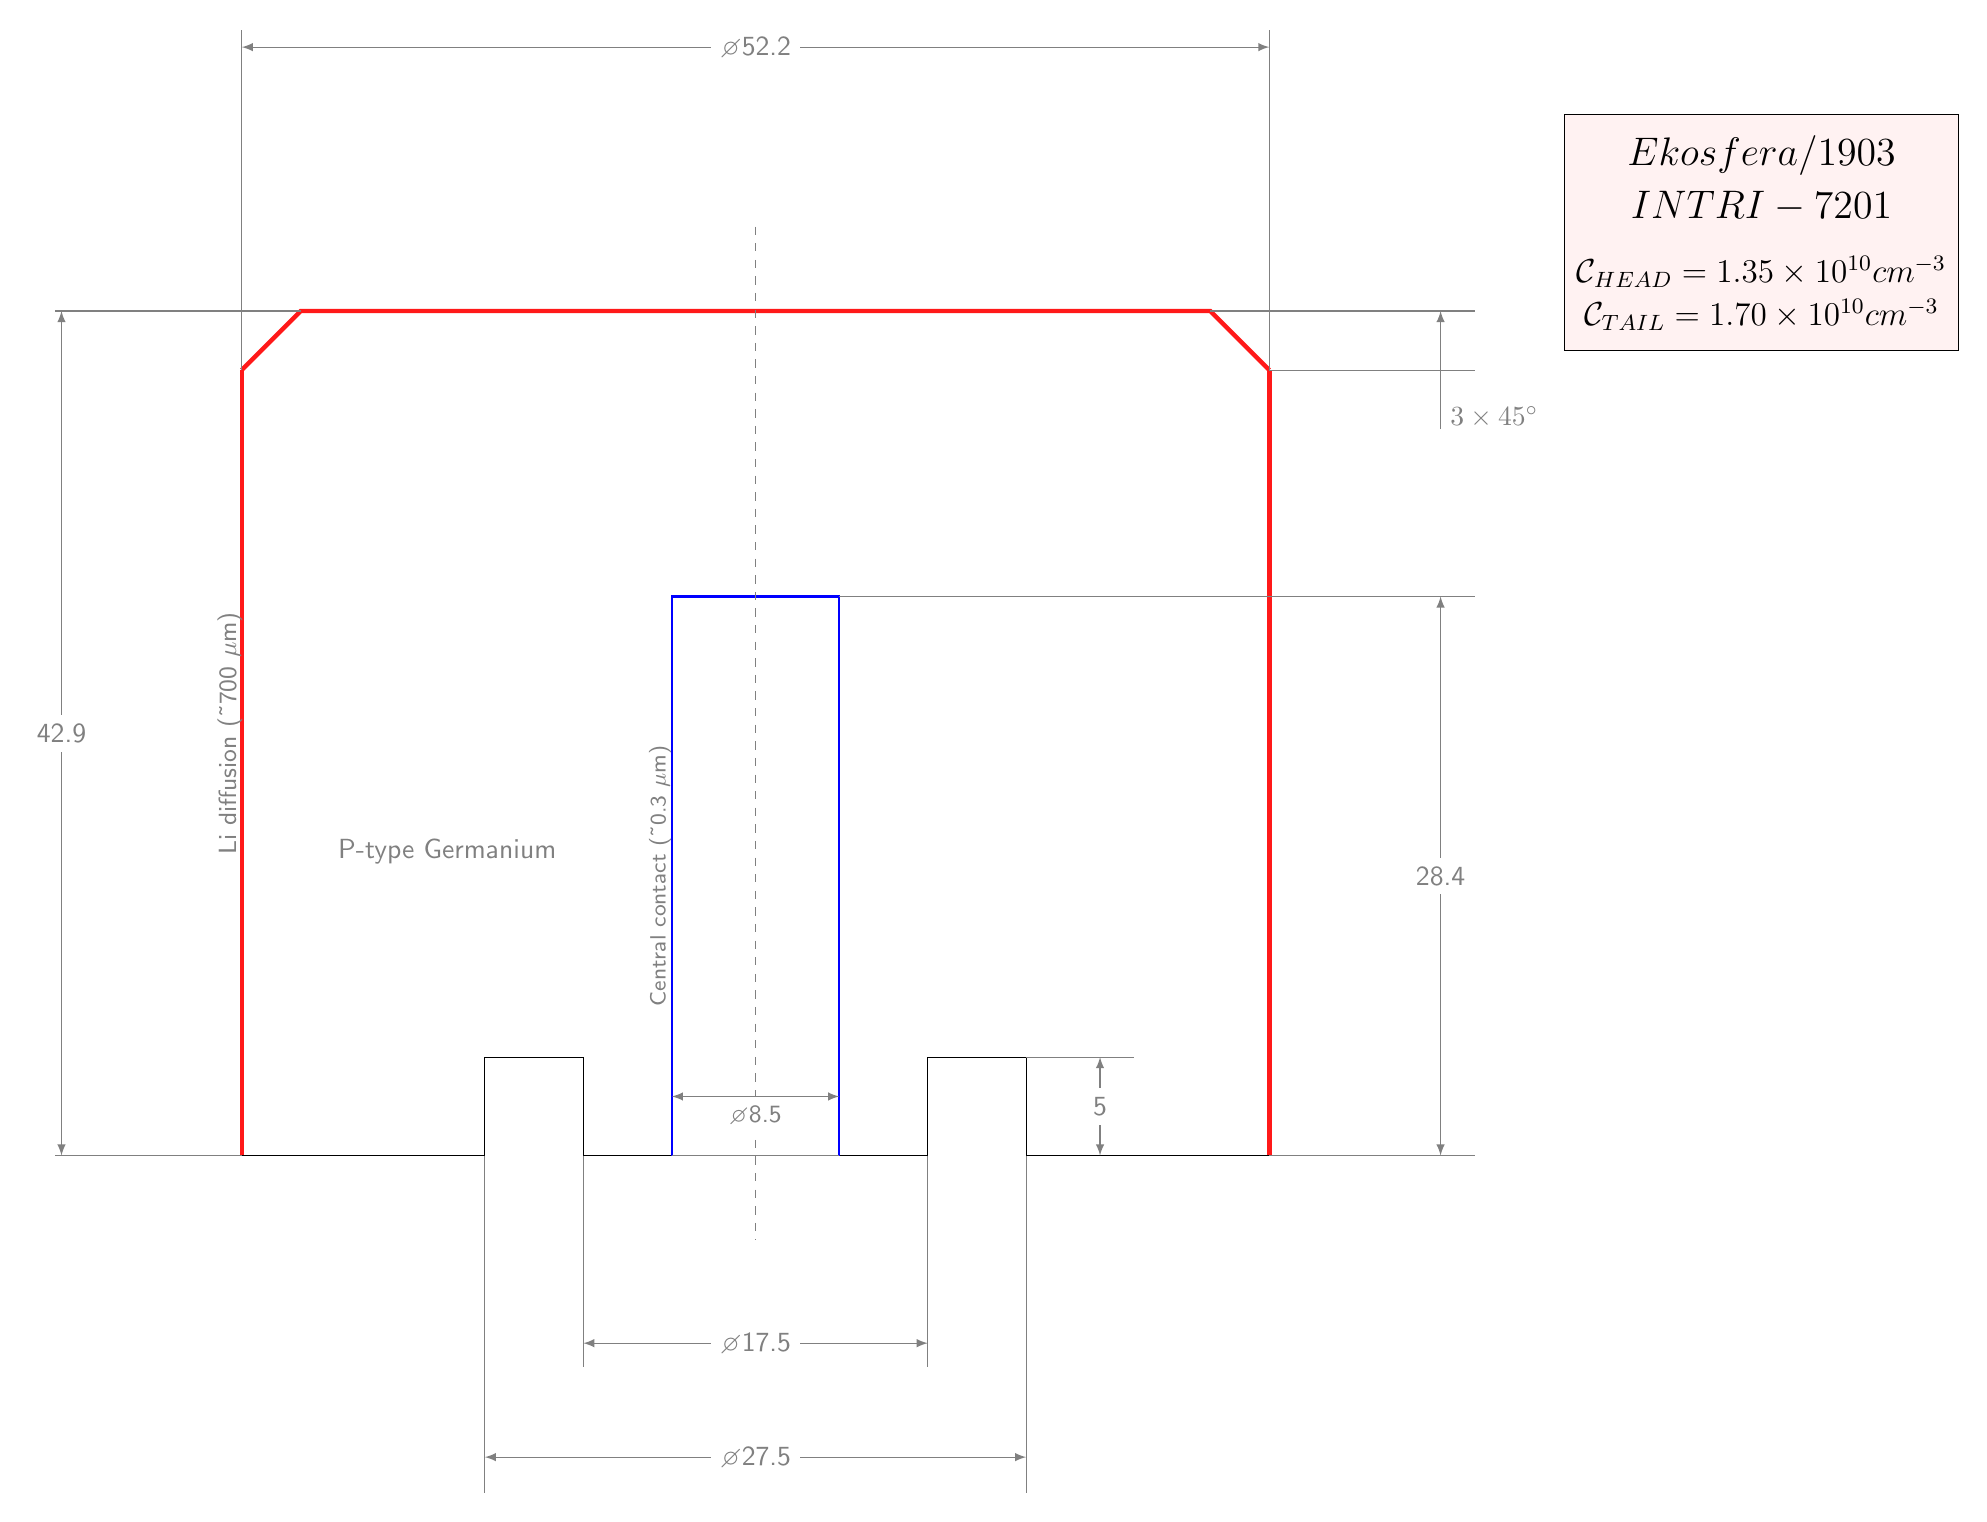
\begin{tikzpicture}
    \draw[lithium] (0,-\Height) -- (0,-\Bullet); %Left wall
    \draw[lithium] (\Diam,-\Height) -- (\Diam,-\Bullet); %Right wall
    \draw[lithium] (0,-\Bullet) -- (\Bullet,0) %bulletize left
     -- (\Diam-\Bullet,0) -- (\Diam,0-\Bullet); %bulletize right
    \draw[thin] (\Diam,-\Height) -- (\Diam/2 +\GrooveExt/2,-\Height) -- (\Diam/2 +\GrooveExt/2,-\Height+\WO) -- 
      (\Diam/2 +\GrooveInt/2,-\Height+\WO) -- (\Diam/2 +\GrooveInt/2,-\Height) -- (\Diam/2 + \FCD /2,-\Height);  %Groove right
    \draw[thin] (0,-\Height) -- (\Diam/2 -\GrooveExt/2,-\Height) -- (\Diam/2 -\GrooveExt/2,-\Height+\WO) -- 
      (\Diam/2 -\GrooveInt/2,-\Height+\WO) -- (\Diam/2 -\GrooveInt/2,-\Height) -- (\Diam/2 - \FCD /2,-\Height);  %Groove left
 
    \draw[thick, blue] (\Diam/2 - \FCD/2,-\Height) -- (\Diam/2 - \FCD/2,-\Height + \Cdepth/\Scale) -- 
    (\Diam/2 + \FCD /2,-\Height + \Cdepth/\Scale) -- (\Diam/2 + \FCD /2,-\Height); %Contact hole

    \draw[gray,thin,opacity=5] (\Diam/2 - \FCD/2,-\Height) -- (\Diam/2 + \FCD /2,-\Height);
    \draw[gray,thin,dashed,opacity=5] (\Diam/2,\Height/10) -- (\Diam/2,-\Height - \Height/10); %Symmetry line
    %--------Captions--------
    \draw (\Diam/2 - \FCD/2 -0.6/\Scale, -\Height + \Cdepth/\Scale/2)node[caption,anchor=center,rotate=90]{\footnotesize Central contact (\char`\~ 0.3 $\mu$m)};
%    \draw (\Diam/2, 0) node[caption,anchor=south]{\small Thin window (\char`\~ 0.3 $\mu$m)};
    \draw (-0.6/\Scale, -\Height*0.5) node[caption,anchor=center,rotate=90]{\small Li diffusion (\char`\~ 700 $\mu$m)};
    \draw (\Diam/5, -\Height/1.5) node[caption,anchor=south]{P-type Germanium};
    %--------Sizes--------
    \draw[dimen] (0,-\Bullet) -- (0,\Height/3);
    \draw[dimen] (\Diam,-\Bullet) -- (\Diam,\Height/3); %---diameter---
    \draw[arrow,<->] (0,\Height/3.2) -- (\Diam,\Height/3.2) node{$\diameter$\pgfmathparse{\Dia}\pgfmathresult};
    %---
    \draw[arrow,<->] (\Diam/2 - \FCD/2, -\Height + 3/\Scale) -- (\Diam/2 + \FCD/2, -\Height + 3/\Scale) node[caption,anchor=north]{\small $\diameter$\pgfmathparse{\Cdiam}\pgfmathresult};
    %---
    \draw[dimen] (\Bullet,0) -- (-\Diam/5.5,0);
    \draw[dimen] (0,-\Height) -- (-\Diam/5.5,-\Height); %---height---
    \draw[arrow,<->] (-\Diam/5.7,0) -- (-\Diam/5.7,-\Height) node{\pgfmathparse{\Hei}\pgfmathresult};
    %---
    \draw[dimen] (\Diam/2-\GrooveInt/2,-\Height) -- (\Diam/2-\GrooveInt/2,-\Height-\Height/4);
    \draw[dimen] (\Diam/2+\GrooveInt/2,-\Height) -- (\Diam/2+\GrooveInt/2,-\Height-\Height/4); %---Groove inner D---
    \draw[arrow,<->] (\Diam/2-\GrooveInt/2,-\Height -\Height/4.5) -- (\Diam/2+\GrooveInt/2,-\Height - \Height/4.5) node{$\diameter$\pgfmathparse{\GrvIn}\pgfmathresult};
    %---
    \draw[dimen] (\Diam/2-\GrooveExt/2,-\Height) -- (\Diam/2-\GrooveExt/2,-\Height-\Height/2.5);
    \draw[dimen] (\Diam/2+\GrooveExt/2,-\Height) -- (\Diam/2+\GrooveExt/2,-\Height-\Height/2.5); %---Groove inner D---
    \draw[arrow,<->] (\Diam/2-\GrooveExt/2,-\Height -\Height/2.8) -- (\Diam/2+\GrooveExt/2,-\Height - \Height/2.8) node{$\diameter$\pgfmathparse{\GrvEx}\pgfmathresult};
    %---
    \draw[dimen] (\Diam-\Bullet,0) -- (\Diam+\Diam/5,0);
    \draw[dimen] (\Diam,-\Bullet) -- (\Diam+\Diam/5,-\Bullet);
    \draw[arrow,->] (\Diam+\Diam/6,-2*\Bullet) -- (\Diam+\Diam/6,0); 
    \draw (\Diam+\Diam/6,-1.8*\Bullet) node[anchor=west,dimen]{$\pgfmathparse{\Bult}\pgfmathresult\times45\degree$}; %Bulletize
    %---
    \draw[dimen] (\Diam/2 +\GrooveExt/2,-\Height+\WO) -- (\Diam/2+\GrooveInt*1.1,-\Height+\WO);
    \draw[arrow,<->] (\Diam/2+\GrooveInt,-\Height+\WO) -- (\Diam/2+\GrooveInt,-\Height) node{\pgfmathparse{\Gdt}\pgfmathresult};
    %---
    \draw[dimen] (\Diam/2+\FCD/2, -\Height+\CDepth) -- (\Diam+\Diam/5,-\Height+\CDepth);
    \draw[dimen] (\Diam,-\Height) -- (\Diam+\Diam/5,-\Height);
    \draw[arrow,<->] (\Diam+\Diam/6,-\Height+\CDepth) -- (\Diam+\Diam/6,-\Height) node{\pgfmathparse{\Cdepth}\pgfmathresult};
    %--- INFO BOX
    \newcommand\Xa{\Diam+15/\Scale}
    \newcommand\Ya{10/\Scale}
    \newcommand\Xb{\Xa+20/\Scale}
    \newcommand\Yb{\Ya-12/\Scale}
    \filldraw[fill=red!5!white, draw=black] (\Xa, \Ya) rectangle (\Xb, \Yb);
    \draw (\Xa+10/\Scale, \Ya-0.6/\Scale) node[anchor=north]{\Large $\Name$};
    \draw (\Xa+10/\Scale, \Ya-3.4/\Scale) node[anchor=north]{\Large $\Crystal$};
    \draw (\Xa+10/\Scale, \Ya-8/\Scale) node[anchor=center]{\large $\mathcal{C}_{HEAD}=\HEAD\times10^{10} cm^{-3}$};
    \draw (\Xa+10/\Scale, \Ya-10.2/\Scale) node[anchor=center]{\large $\mathcal{C}_{TAIL}=\TAIL\times10^{10} cm^{-3}$};
    %---
    %\draw[dimen] (\Diam-\Bullet,0) -- (\Diam*1.2,0);
  \end{tikzpicture}

\end{document}
